\section{Results \& Statistical Analyses}
\subsection{Spatio-temporal asynchrony and post-error slowing}

In the synchronous trials, participants reached the target on average after 1.04 (sd = .19) seconds following the spawn on the table at one of three possible location. Increasing the collider size by a factor of 3.5 resulted, as expected, in a shortened reaction time of .73 (sd = .12) seconds, see figure \ref{velocity} D. Hence in manipulated trials, an asynchrony of ~300ms led to a perturbed spatio-temporal congruence. The velocity profile in both conditions exhibited a narrow peak during outward reaching with a peak magnitude of ~.6 m/s and a broader and lower peak retracting the hand, \ref{velocity} C top.

% Frage: wenn vel profiles mit movement onset aligned dann sollten evtl. kurven gleich sein, es sei denn es gibt einen "kontinuierlichen" rekalibrationseffekt ist in den syncs. mit drin
% im idealfall ist der rekalibrationseffekt 1/4 der 300ms
% Optimierungsprozess um den RMSE bei rekalibration zu optimieren
% mallot VR noise adaptation

\begin{figure}[t]
  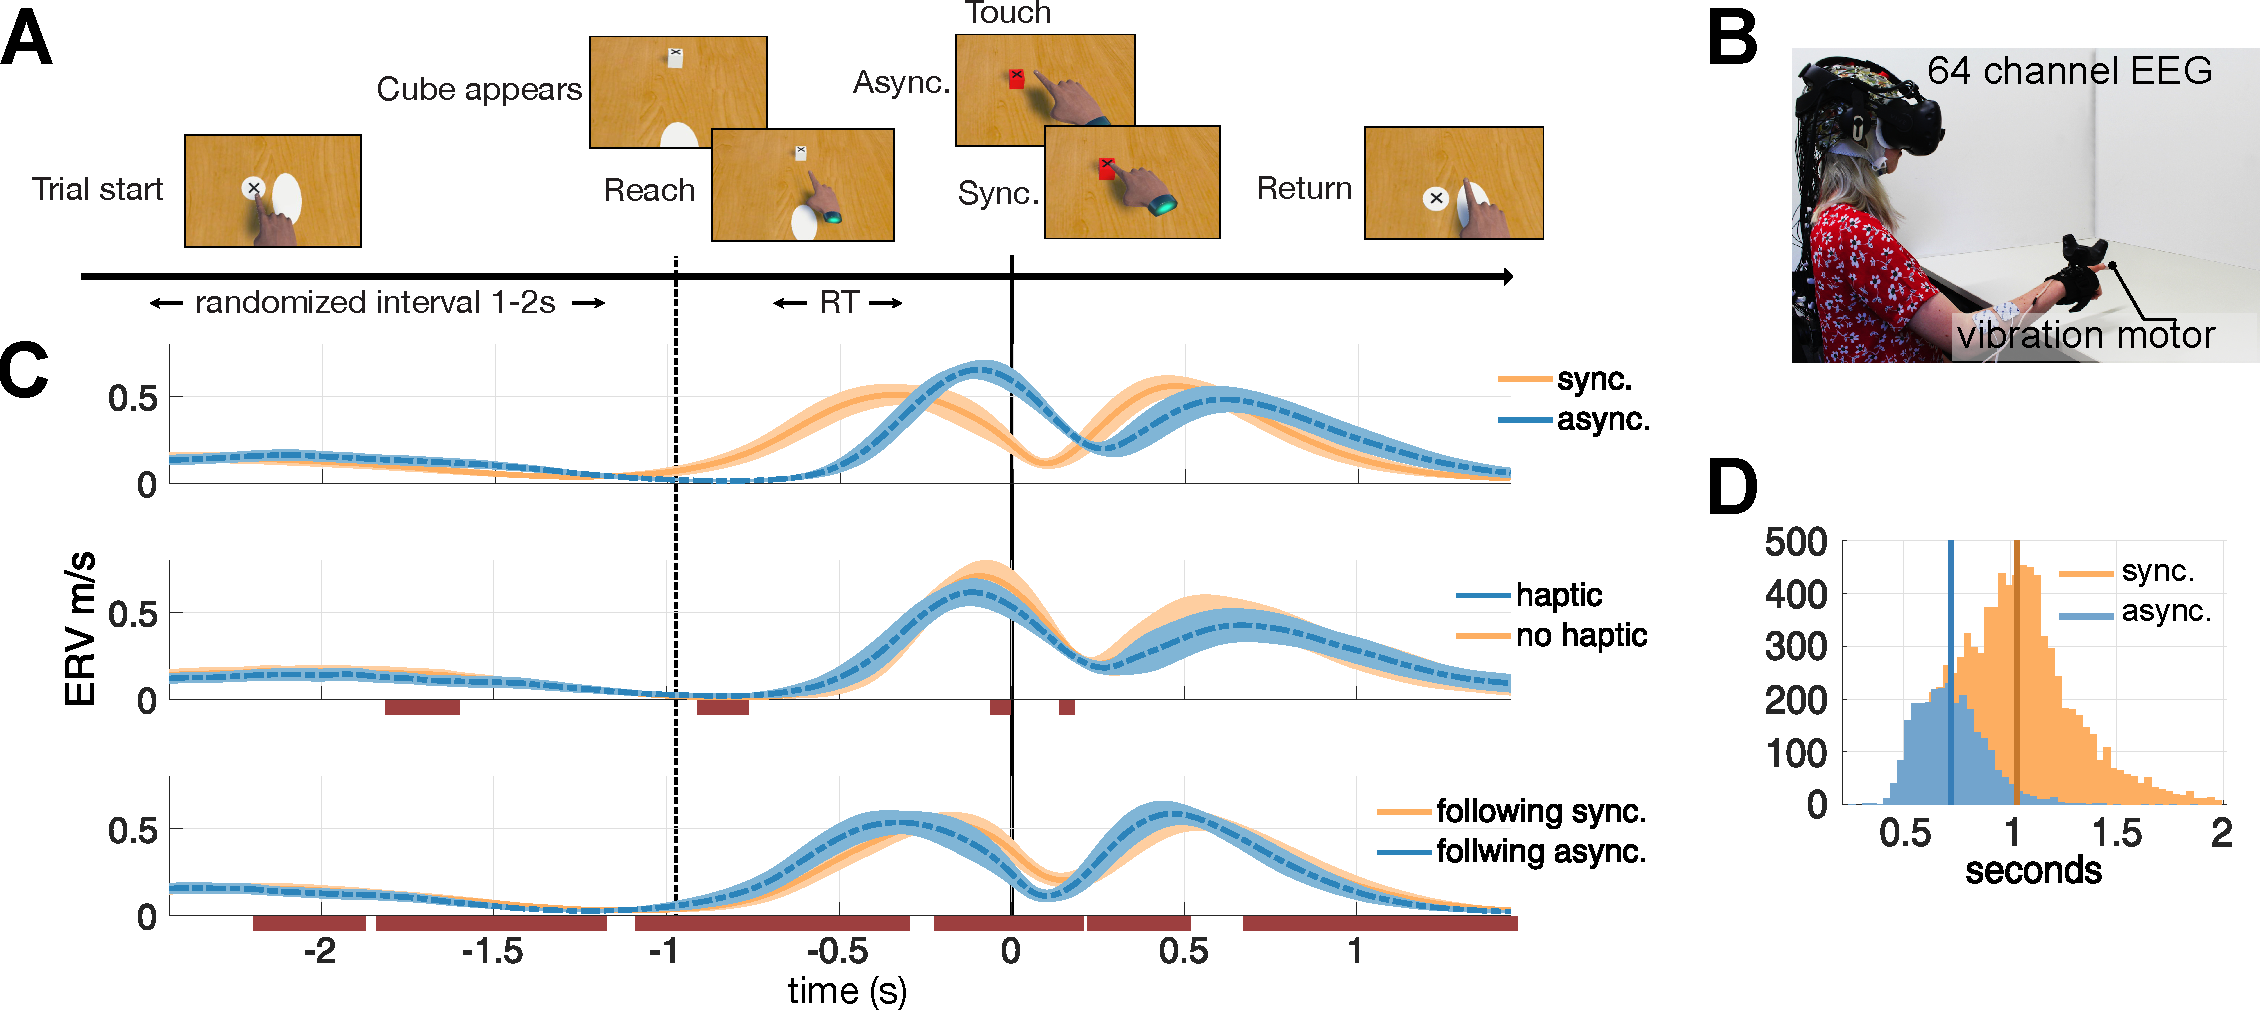
\includegraphics[width=\textwidth]{figures/fig1_behavior.pdf}
  \caption{Task Structure and event-related velocity (ERV). \textbf{A} Participants were instructed to reach to an appearing cube on a desk in front of them. \textbf{B} Virtual reality setup with 64 channel electrode montage, electrode spacers and rigid body tracker on the hand. Under the fingertip of the index finger, a vibration motor. \textbf{C} Grand-average magnitudes of velocity with 95\% confidence interval and contrasting synchronicity (top), haptic feedback (middle) and whether the preceeding trial was asynchronous (bottom), aligned at the touch feedback. \textbf{D} Time between object spawn and selection, reaction time, for synchronicity.}
  \label{velocity}
\end{figure}

The addition of a haptic sensation while touching the virtual objects (by means of vibrotactile stimulation) led participants to generally move their hand slower during the whole trial, see \ref{velocity} C middle row. Participants started their outward movement earlier and their outward peak magnitude was lower when approaching the target (for example at 50 ms preceding object selection, $t_{18} = -2.14, P = .03$). Following trials with spatio-temporal asynchrony, movement behavior was altered in the next trial. An earlier movement onset with a broader peak and immediate retraction following object select was observed (for example at 100 following object selection, $t_{18} = -17.24, P = 0$). Taken together, the task introduced spatio-temporal asynchrony, with rendered vibrotactile feedback as well as the asynchrony impacting future reaching movement characteristics.